
\chapter{Testing and Evaluation}
\label{chap:eval}
\lhead{\emph{Project Testing}}

To validate the effectiveness of the NoteReader application, a comprehensive testing process was conducted. A variety of sample files in different formats were used to assess the system’s ability to meet its functional and non-functional requirements. These files included PDFs, DOCX, PPTX, EPUB, and HTML documents, and enabled rigorous evaluation of file parsing, rendering fidelity, and performance \ref{fig:sample_files}.


\section{Requirements}

    \subsection{Functional Requirements}
            \subsubsection{
            The system shall provide a split-view interface to allow users to view documents and take notes simultaneously}
            \textbf{Status: Fulfilled}   \newline
            The application successfully implements a split-view interface, where the document is displayed in the left pane and a markdown-compatible note editor appears in the right pane. \ref{fig:notereader_twopane}.
            
            \subsubsection {
            The system shall support the import and display of PDF, EPUB, DOCX, and PPTX files}            
            \textbf{Status: Fulfilled}   \newline
            The application supports a wide range of file types including PDF, DOCX, DOC, PPTX, EPUB, and HTML. These formats were selected based on their prevalence in academic environments and have been verified to load and render successfully and true to intent.
            
            \subsubsection {
            The system shall allow users to link notes to specific pages or sections of the source document.}            
            \textbf{Status: Fulfilled}  \newline
            The system correctly associates notes with specific pages of the source document. Each note is saved in a file named to reflect its corresponding page number, enabling automatic retrieval and display when users navigate to a particular page.
            
            \subsubsection {
            The system shall support searching and filtering of notes and documents using tags, keywords, and categories.}
            \textbf{Status: Not Fulfilled}  \newline
            This functionality was not implemented due to time constraints and has been deferred to future development cycles.
            
            
            \subsubsection {
            The system shall support exporting notes in plain text format for use in other applications.}
            \textbf{Status: Fulfilled}  \newline
            All notes are stored in markdown format (.md), enabling seamless export to and reuse in third-party applications such as Obsidian.
            
            
            \subsubsection {The system shall enable users to sync notes to cloud storage providers like GitHub using version control.}
            \textbf{Status: Not Fulfilled}  \newline
            Version-controlled synchronization using platforms like GitHub was intended but not implemented due to limited development time.

            
            \subsubsection {The system shall allow users to tag and categorize notes for efficient organization and retrieval.}
            \textbf{Status: Not Fulfilled}  \newline
            Although planned, tagging and categorization features were not developed in this phase of the project.
            


    \subsection{Non-Functional Requirements}
        \subsubsection { Performance: The system shall load and display documents without noticeable wait times on standard modern devices.}
        \textbf{Status: Partially Fulfilled}
        This Requirement has been partially fulfilled. PDF files are very quick to load, but the requirement to convert other document types can result in noticeable wait times. EPUB is especially long with the sample document taking approximately 5 seconds to load an ebook with 115 pages. 

        Once the document is converted however, it is very quick to navigate between pages. Pagination and lazy loading was implemented to ensure the impact on memory resources is kept to a minimum and ensure good performance. 


        \subsubsection { Usability: The user interface shall be intuitive, with clear user experience flows. }
        \textbf{Status: Fulfilled}

        This requirement is slightly more subjective, though I did design the application with this in mind, and would consider it to have been fulfilled. 

        I implemented the program in a manner which requires as few clicks as possible to enter a file. importing a document is as simple as selecting "import", then selecting the name of the document. 

        While in the reader view, The left pane shows the document, while the right shows the note taking window. The note taking window is coloured with a yellow tint, to evoke the thought of a traditional sticky note, so the purpose of the pane is immediately clear. 

        Buttons are large, and have icons that indicate their purpose, such as a magnifying glass for zooming. 


        \subsubsection { Scalability: The system shall support large document files (over 25mb), and offer alternative synchronization methods for these files. }
        \textbf{Status: Deferred}
        Although large files can be imported, advanced synchronization strategies for large datasets (e.g., LFS for Git) are not yet implemented and remain a future goal.

        
        \subsubsection { Portability: The system shall support cross-platform functionality on Windows, macOS, Linux, and mobile devices.}        \textbf{Status: Not Yet Fulfilled}
        While the application has not yet been deployed on multiple platforms, it is architected using Kotlin Multiplatform, enabling straightforward extension to additional targets in future iterations.

    
        \subsubsection { Reliability: The system shall gracefully handle unexpected crashes to prevent data loss by saving notes in real-time and automatically restoring the last working state upon restart.}
        \textbf{Status: Fulfilled}
        All notes are saved in real time as the user edits them.
        A persistent application state is maintained using a JSON file, which is read on application launch to restore the last session \ref{fig:state_json}

         
        \subsubsection { Maintainability: The system shall be modular to allow for easy updates and addition of new features.}
        \textbf{Status: Fulfilled}

        The application employs a Model-View-Controller (MVC) architecture, supporting clean separation of concerns. 
        
        Views are built in Compose, allowing individual components to be replaced or extended with minimal coupling. 
        
        New document format support can be easily added by inserting appropriate logic modules into the existing flow.
        

\begin{figure}
    \centering
    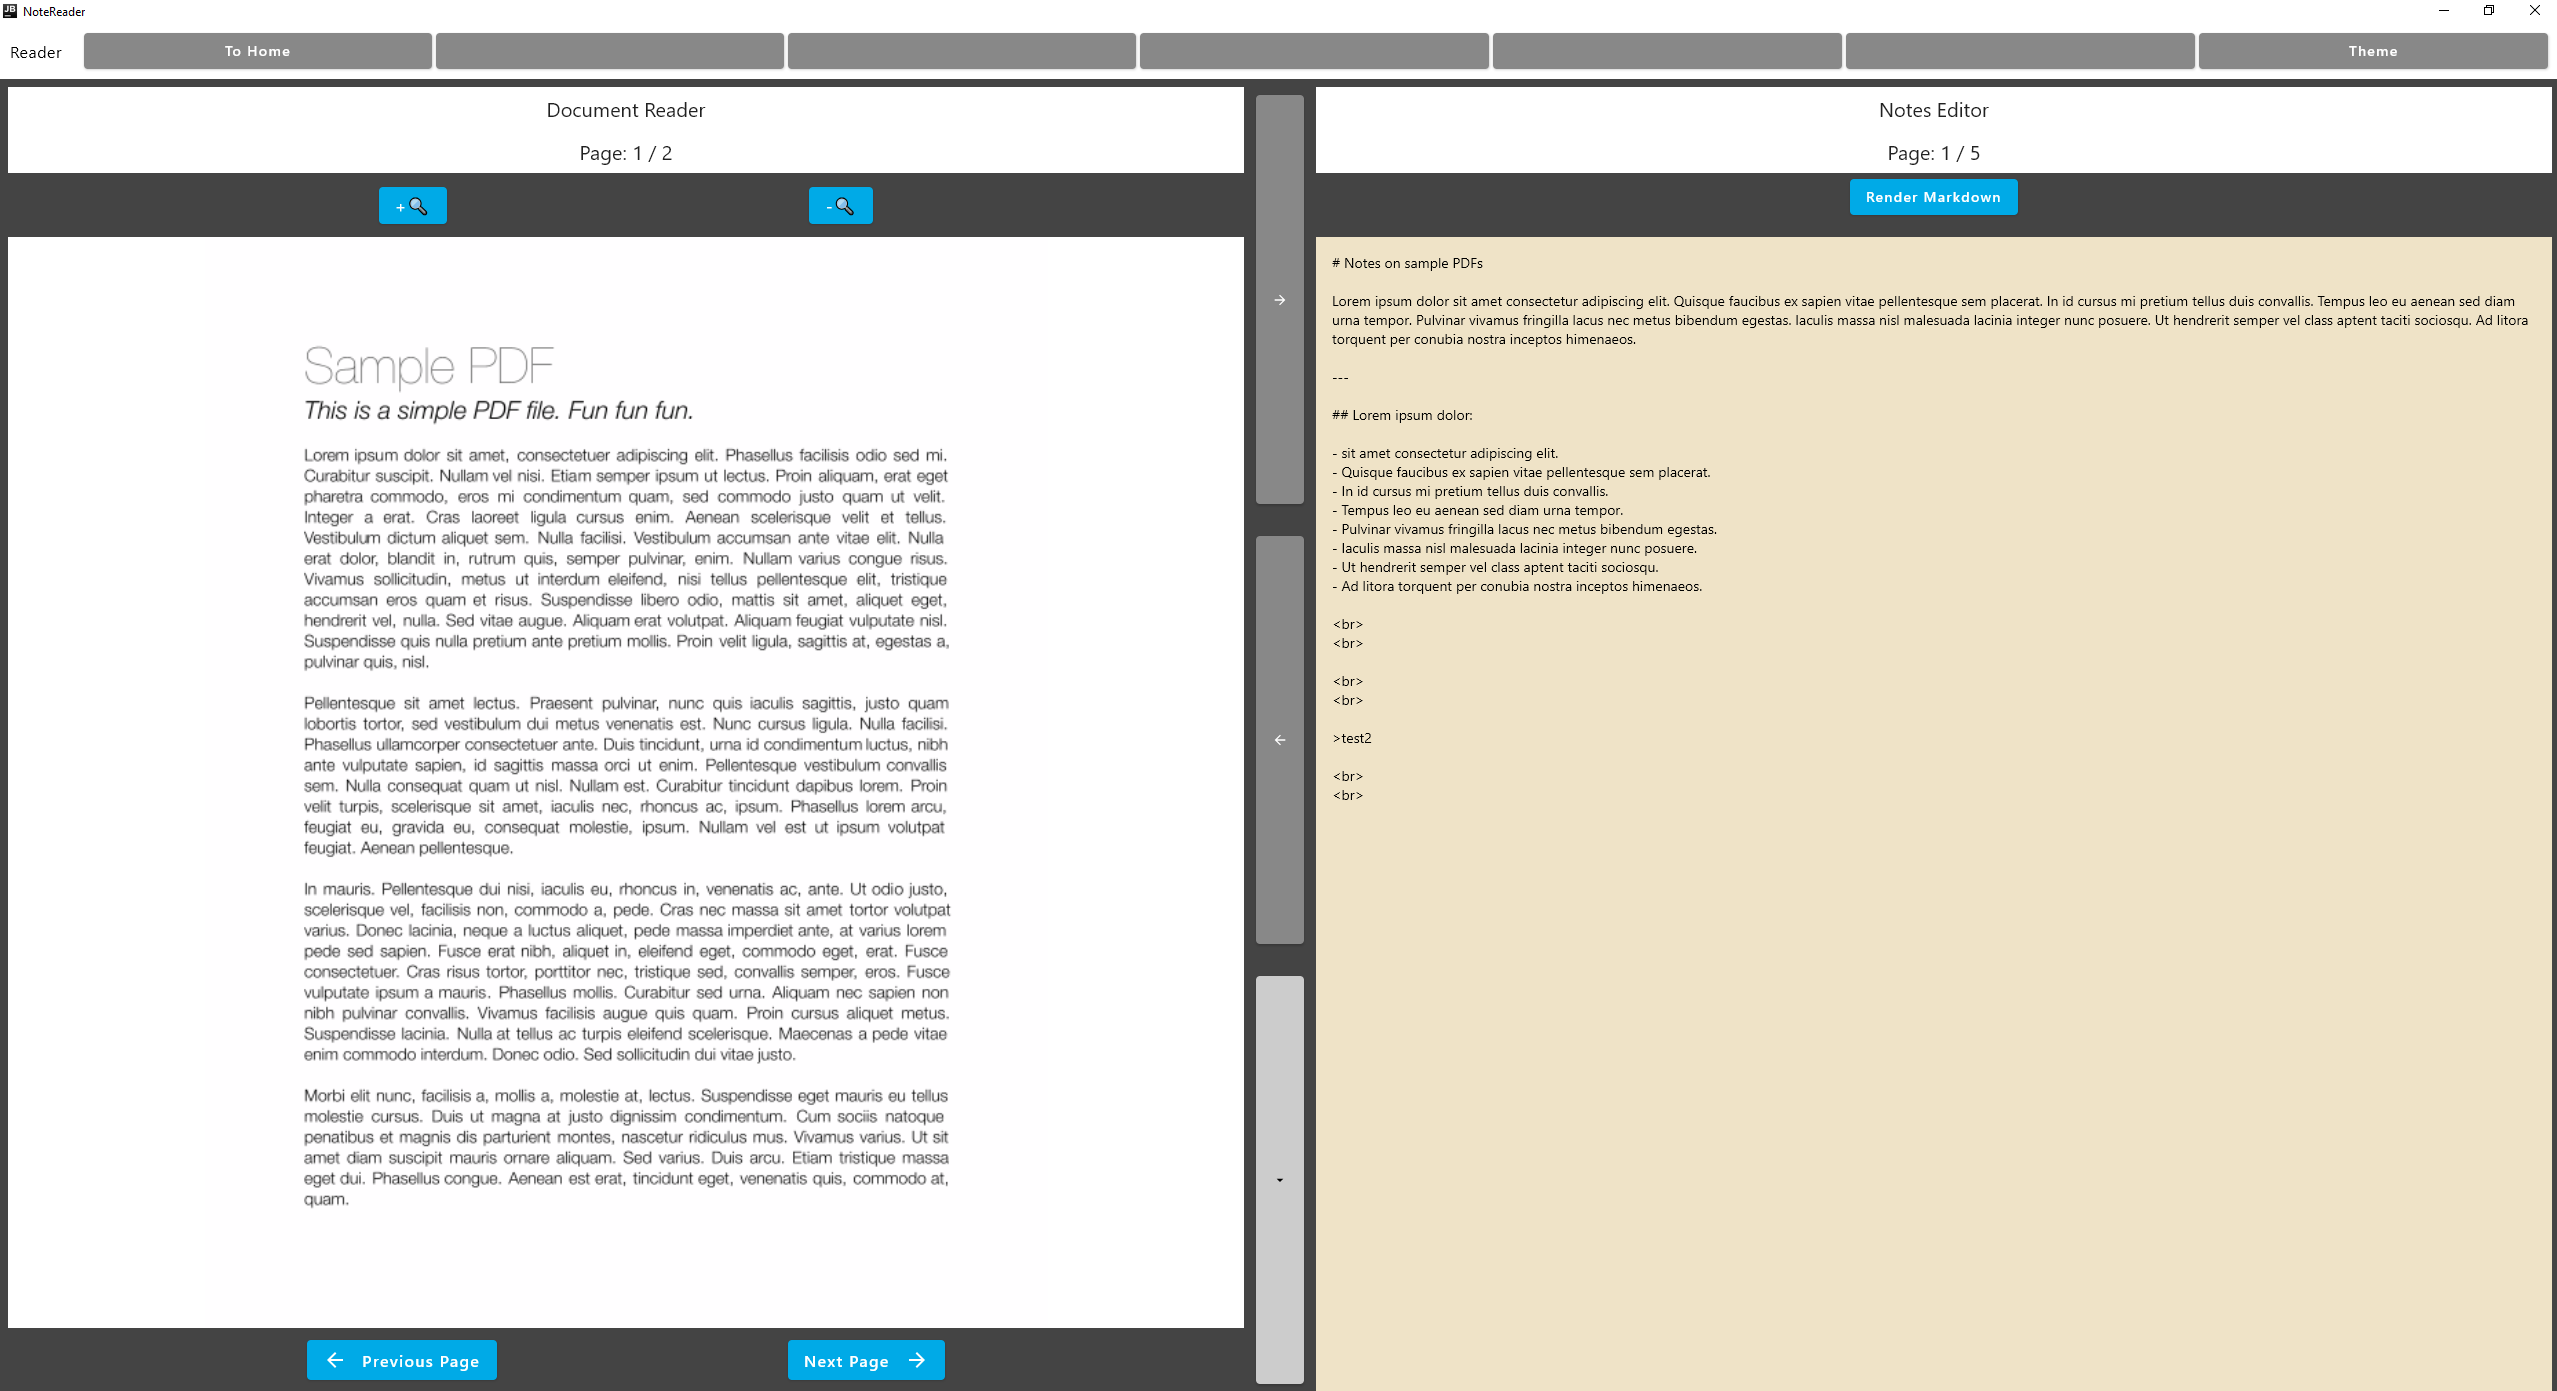
\includegraphics[width=1\linewidth]{image.png}
    \caption{A screenshot of the NoteReader Application, showing the two pane layout}
    \label{fig:notereader_twopane}
\end{figure}    

\begin{figure}
    \centering
    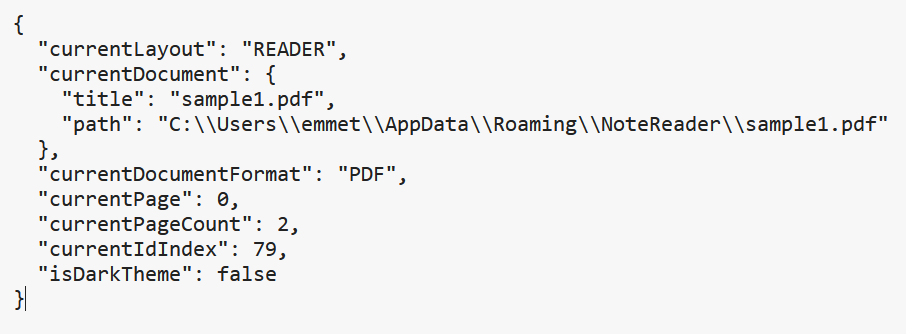
\includegraphics[width=1\linewidth]{state_json.png}
    \caption{Sample Program State in Json Format}
    \label{fig:state_json}
\end{figure}

\begin{figure}
    \centering
    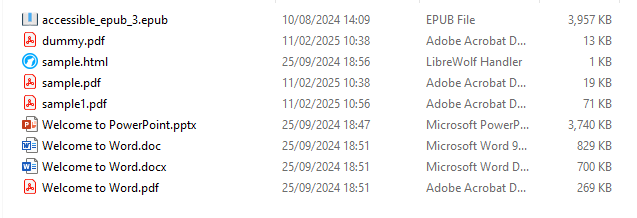
\includegraphics[width=1\linewidth]{sample_files.png}
    \caption{Sample Files used for testing}
    \label{fig:sample_files}
\end{figure}

% The goal of this chapter is an objective evaluation of the final system. The evaluation must be quantitative and not qualitative. You may perform qualitative evaluation but this should not form the basis of the main conclusions you derive from the evaluation. This evaluation, where possible, should be comparative, i.e. you should evaluate your system against a commercially available system and/or system detailed in a research publication. You should demonstrate operational testing of the project using real or contrived data sets to evaluate aspects of the project not encompassed in the software testing (e.g. quantify how well does your project achieved the overall goal). 
% \begin{itemize}
%     \item For software based projects this will include, but should not be limited to, evaluation of non-functional requirements.
%     \item For infrastructural projects this testing should include system/network KPI analysis.
%     \item For analysis based projects (ML, malware or other) this may include model evaluation or YARA rule validation, for example.
%     \item For management projects, where software testing or infrastructure testing may not be in scope, the test process for the system is expected to be more rigorous and well described than a project incorporating significant development work.
% \end{itemize} 

% Some suggested sections (the nature of this chapter should be discussed in detail with your term 2 supervisor):

\section{Metrics}
% Identify and describe the metrics you used to evaluate your project. You should have identified some of these in the research phase report but will detail these as you progress through the design.

\begin{itemize}
    \item \textbf{Feature Completeness}: Whether each intended feature was implemented and functioned as expected during manual use.
    \item \textbf{File Compatibility}: Evaluation of whether a variety of common document formats (PDF, DOCX, EPUB, PPTX, HTML) could be opened, rendered, and navigated.
    \item \textbf{Stability and Recovery}: Observations of the application's behaviour when reopened after closing mid-session, including state persistence, and real time saving of notes.
    \item \textbf{Document-to-Note Linking Accuracy}: Inspection of whether notes correctly reloaded for their associated page, and validating that files are created and sorted appropriately. 
\end{itemize}

These observational metrics provided a practical basis for assessing whether NoteReader met its intended goals and provided a usable experience for real-world document annotation workflows.



\section{System Testing}
% Describe the experimental setup for each metric, and how you obtained the measurements. Describe the inputs for each experiment

System testing was conducted manually, using a range of sample files selected to represent typical academic study materials. The goal was to validate the system’s ability to import, render, and annotate documents across a variety of formats. The following test process was followed:

\begin{itemize}
    \item \textbf{Document Import and Rendering}: Sample files (PDF, EPUB, DOCX, PPTX, HTML) were imported to check if they rendered correctly in the split-view layout. Each file was inspected for formatting integrity and legibility.
    \item \textbf{Note Creation and Retrieval}: Notes were created for specific pages, then navigation was tested to confirm that the correct note appeared when returning to that page.
    \item \textbf{Session Persistence}: The program was closed mid-session and reopened to test whether the last viewed document and notes were restored successfully. Crashes were simulated by ending execution of the program directly in the Android Studio IDE. 
    \item \textbf{File System Inspection}: The folder structure and file output were manually verified to confirm that notes were stored in plain-text markdown format and logically organized per document.
\end{itemize}

While these tests did not produce numeric results, they provided confidence that core functionality worked as intended under normal usage conditions.

\section{Results}
% Summarise the output data, and the statistical or other techniques to deduce your results. Summarise your results, including tables or graphs as appropriate with a brief description of each. here possible, compare your results with other products/systems. Identify any possible threats to the validity of your results, and discuss each briefly here (you will discuss in more detail in the next chapter).

The manual testing process confirmed that the core features of NoteReader function as expected across a range of sample documents. Below is a summary of observed results:

\begin{itemize}
    \item \textbf{File Compatibility}: All tested formats PDF, DOCX, PPTX, EPUB, and HTML were successfully rendered using the PDF conversion pipeline. Formatting was preserved in all cases.
    \item \textbf{Note Linking}: Notes were correctly saved per page and reloaded without error. 
    \item \textbf{State Restoration}: On restarting the application, the previous session's document and page state were restored, confirming that persistence was functioning as designed. when simulating crashes, all notes were verified to have saved correctly. 
    \item \textbf{Interface Stability}: In the final version no crashes were encountered during normal use.
\end{itemize}

\subsection{Limitations}
\begin{itemize}
    \item A lack of automated testing may lead to blind spots over time. Manual testing was appropriate for the graphical elements of the application, but subsequent development cycles should focus on unit testing as a priority. 
    \item Testing was conducted only on two devices (Windows 10 and Windows 11).
    \item No formal load or performance testing was conducted. While considerations were made to performance, such as the implementation of lazy loading and pagination, observations of responsiveness were subjective.
\end{itemize}